\documentclass[a4paper,10pt]{article}
\usepackage[utf8]{inputenc}
\usepackage[margin=1.5cm, bottom=2cm]{geometry}
\usepackage{fancyhdr}
\usepackage[dvipsnames]{xcolor}
\usepackage{enumitem}
\usepackage{xcolor}
\usepackage[table]{xcolor}
\usepackage{makeidx}
\usepackage[most]{tcolorbox}
\setlength{\parindent}{0pt}
\newtcolorbox{osservazioni}{
  colback=gray!8,    % sfondo grigio chiaro
  colframe=white,      % nessun bordo
  arc=2mm,            % angoli smussati
  boxrule=0pt,        % spessore bordo 0
  fontupper=\footnotesize,
  left=2mm, right=2mm, top=2mm, bottom=2mm,
  before skip=7pt,   % niente spazio prima
  after skip=15pt     % niente spazio dopo
}
\newtcolorbox{osservazioni2}{
  colback=ForestGreen!4,    % sfondo grigio chiaro
  colframe=white,      % nessun bordo
  arc=2mm,            % angoli smussati
  boxrule=0pt,        % spessore bordo 0
  fontupper=\footnotesize,
  left=2mm, right=2mm, top=2mm, bottom=2mm,
  before skip=7pt,   % niente spazio prima
  after skip=15pt     % niente spazio dopo
}
\pagestyle{fancy}
\usepackage{tikz}
\usetikzlibrary{automata, positioning}
\pagestyle{fancy}

\usepackage{makeidx}

%%%%%%%%%%%%%%%%%%%
\newcommand{\DocType}{Esercitazione} % o "Eserciziario"
\newcommand{\FullTitle}{\DocType\ \EsercitazioneNum}

\newcommand{\Header}{
\noindent
  \small \textbf{Computabilità, Complessità e Logica - a.a. 2025/26} \hfill \textbf{\FullTitle} \\[0.2cm]
  \scriptsize Matteo Liotta, \texttt{matteo.liotta@studenti.units.it} \hfill \Data \\[0.2cm]
  \noindent\makebox[\linewidth]{\rule{\linewidth}{0.4pt}} \\[0.3cm]}

\newcommand{\NewPageHeader}{
  \vfill
  \noindent\makebox[\linewidth]{\rule{\linewidth}{0.4pt}}
  \newpage
  {\Header}
}
%%%%%%%%%%%%%%%%%%%
\newcommand{\EsercitazioneNum}{03}
\newcommand{\Data}{13/12/2025}
%%%%%%%%%%%%%%%%%%%

% Numero di pagina in basso al centro
\fancyhf{}
\fancyfoot[C] \thepage
\renewcommand{\footrulewidth}{0pt} % niente linea in basso
\renewcommand{\headrulewidth}{0pt} % niente linea in alto

\begin{document}
\footnotesize  % font generale più piccolo

\noindent
\small \textbf{Computabilità, Complessità e Logica - a.a. 2025/26} \hfill \textbf{Approfondimento \EsercitazioneNum} \\[0.2cm]
\scriptsize Matteo Liotta, \texttt{matteo.liotta@studenti.units.it} \hfill \Data \\[0.2cm]

\noindent\makebox[\linewidth]{\rule{\linewidth}{0.4pt}} \\[1cm]


\noindent\Large \textbf{Approfondimento \EsercitazioneNum}: \textit{Dalla logica proposizionale alla logica dei Predicati}\\[0.1cm]
%\\[0.4cm]



\small

\underline{\textbf{Logica Proposizionale}}\\

L'introduzione della logica proposizionale ci permette di descrivere formalmente problemi tramite l'utilizzo di variabili su dominio booleano. In particolare, abbiamo introdotto variabili della forma: $$X\quad t.c.\quad \alpha(X)\in \{0,1\}$$ che è possibile immaginare come una \textit{affermazione}, che, come tale, ammette un valore di verità. Ogni variabile, come è stato possibile osservare anche durante la risoluzione di esercizi, codifica una risposta o affermazione su qualsiasi oggetto. Se supponiamo di voler descrivere un'osservabile dell'oggetto, possiamo quindi ricorrere all'utilizzo di una affermazione costruita proprio intorno ad esso. Un esempio può essere concentrarsi sul parlare di azioni o proprietà dei giorni, relativamente alla situazione meteorologica che essi possiedono. Alcuni esempi:

\begin{center}
    \textit{$A:=$ Il cielo è nuvoloso}\\
    \textit{$B:=$ Il cielo è soleggiato}\\
    \textit{$C:=$ Sta piovendo}
\end{center}
Dove all'affermazione complessa: 
\begin{center}
    $\phi := C \rightarrow A\quad\quad$
    \textit{Il fatto che \textbf{fuori è nuvoloso} implica che \textbf{fuori sia nuvoloso}}
\end{center}
può essere associato un valore di verità, così come per ciascuna delle variabili. Ammette un potenziale valore di verità $1$ o $0$, garantendoci la possibilità di parlare di alcune situazioni attraverso una formula booleana.
$$\alpha\models \phi$$ può essere $$\alpha :=\{A\leftarrow 0, C\leftarrow1\}$$
Parlare di diversi giorni e di ciascuna delle relative casistiche, ci porta obbligatoriamente dell'introduzione di una affermazione che la caratterizzi per ciascuna di tali combinazioni, incrementando chiaramente il numero di variabili.\\
Un esempio di ciò, in cui possibile chiaramente quantificare la natura del problema è quello del Sudoku: possiamo associare ad una variabile la descrizione di un'osservabile per ciascuna specifica cella. La natura però dell'associazione della caratteristica e l'oggetto che ne gode, è notevolmente limitante in molti contesti: ogni variabile descriverebbe una caratteristica, affermazione o risposta chiara e non parametrica, su un singolo oggetto, da cui impossibile generalizzare. Per parlare, come avvenuto nel caso del Sudoku, di ciascuna cella e codificare la frase: 
\begin{center}
    \textit{La cella $(i,j)$ contiene il numero $k$}
\end{center}
siamo dovuti ricorrere all'impiego di \textbf{729} variabili, una per ciascuna casistica:
$$X_{i,j,k}\quad \quad i,j,k\in\{1,...,9\}$$
Come ad esempio:
\begin{center}
    \textit{$X_{3,7,2}$ = La cella $(3,7)$ contiene il numero $2$}\\[1cm]
\end{center}

\underline{\textbf{Logica dei Predicati}}\\

Perché allora non possiamo svincolare la caratterizzazione dall'oggetto caratterizzato? Ecco dunque l'idea alla base della logica dei predicati: svincolare l'elemento $x$ appartenente ad un dominio di interesse $D$ da una sua eventuale caratterizzazione -detta predicato- $P$. In questo modo, abbiamo, ad esempio, la possibilità non solo di parlare di diversi \textit{aspetti}  per un fissato elemento del dominio, ma anche introdurre dei quantificatori che permettano di generalizzarne il comportamento, limitando il numero di variabili e semplificando la scrittura delle formule.

$$\exists x.A(x)\rightarrow B(x)$$

\NewPageHeader

Data questa formula, possiamo scegliere di osservarla sul nostro dominio dei giorni, così da svincolare la variabile dell'osservazione dalla \textit{giorno} situazione metereologica che esso possiede.

\begin{center}
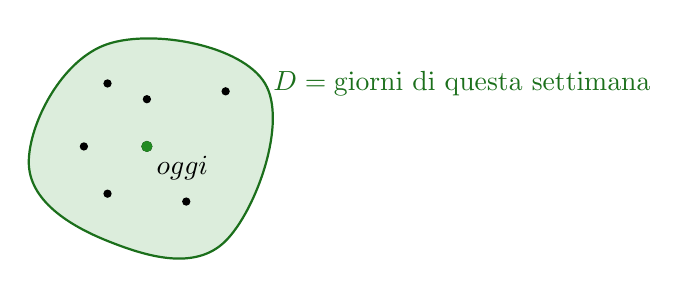
\begin{tikzpicture}

    % 1. Definizione dell'area (riempimento)
    % Usiamo 'fill' con un colore leggero e un po' di trasparenza
    \fill[ForestGreen!20, opacity=0.8] plot [smooth cycle, tension=0.7] coordinates {
        (0,0) (1,1.5) (3,1) (2.5,-1) (1,-1)
    };

    % 2. Disegno del contorno
    % Usiamo le stesse coordinate per disegnare il bordo
    \draw[thick, ForestGreen!80!black] plot [smooth cycle, tension=0.7] coordinates {
        (0,0) (1,1.5) (3,1) (2.5,-1) (1,-1)
    };

    % 3. Etichetta del dominio
    \node[ForestGreen!80!black] at (5.5, 1) {$D=\text{giorni di questa settimana}$};

    % 4. Aggiunta di punti interni

    \fill[black] (1.5, 0.2) circle (2pt);
    %\node[below right] at (.5, 0.3) {$z_2$};

    % Punto P
    \fill[ForestGreen] (1.5, 0.2) circle (2pt);
    \node[below right] at (1.5, 0.2) {$oggi$};

    % Altro punto Q
    \fill[black] (2, -0.5) circle (1.5pt);
    \fill[black] (1, -0.4) circle (1.5pt);
    \fill[black] (0.7, 0.2) circle (1.5pt);
    \fill[black] (1, 1) circle (1.5pt);
    \fill[black] (1.5, 0.8) circle (1.5pt);
    \fill[black] (2.5, 0.9) circle (1.5pt);
    %\node[right] at (2, -0.5) {$z_1$};

\end{tikzpicture}
\end{center}

Allora le caratterizzazioni -i.e. i predicati-, altro non sono che dei sottoinsiemi del dominio di interesse: 

\begin{center}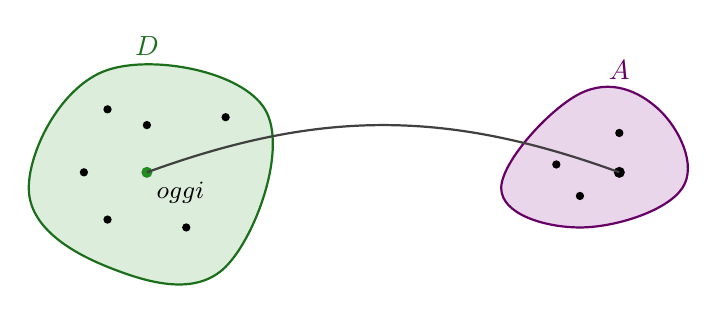
\begin{tikzpicture}

    % ==========================================
    % 1. DOMINIO D (A SINISTRA)
    % ==========================================
    
    % Area
    \fill[ForestGreen!20, opacity=0.8] plot [smooth cycle, tension=0.7] coordinates {
        (0,0) (1,1.5) (3,1) (2.5,-1) (1,-1)
    };
    \draw[thick, ForestGreen!80!black] plot [smooth cycle, tension=0.7] coordinates {
        (0,0) (1,1.5) (3,1) (2.5,-1) (1,-1)
    };
    \node[ForestGreen!80!black] at (1.5, 1.8) {$D$};

    % Punti di D
    % NOTA: Aggiungo "coordinate (nome)" per ricordarli dopo
    \fill[ForestGreen] (1.5, 0.2) circle (2pt) coordinate (puntoOggi); 
    \node[below right] at (puntoOggi) {\small $oggi$};

    \fill[black] (2, -0.5) circle (1.5pt);
    \fill[black] (1, -0.4) circle (1.5pt);
    \fill[black] (0.7, 0.2) circle (1.5pt);
    \fill[black] (1, 1) circle (1.5pt) coordinate (altroPunto); % Un altro punto a caso
    \fill[black] (1.5, 0.8) circle (1.5pt);
    \fill[black] (2.5, 0.9) circle (1.5pt);


    % ==========================================
    % 2. INSIEME A (A DESTRA)
    % ==========================================
    % Usiamo uno SCOPE traslato di 6cm a destra
    
    \begin{scope}[xshift=6cm] 
        % Area
        \fill[Purple!20, opacity=0.8] plot [smooth cycle, tension=0.7] coordinates {
            (0,0) (1,1.2) (2,1) (2.3,0) (1,-0.5)
        };
        \draw[thick, Purple!80!black] plot [smooth cycle, tension=0.7] coordinates {
            (0,0) (1,1.2) (2,1) (2.3,0) (1,-0.5)
        };
        \node[Purple!80!black] at (1.5, 1.5) {$A$};

        % Punti di A
        \fill[black] (1.5, 0.2) circle (2pt) coordinate (destinazione1);
        \fill[black] (1, -0.1) circle (1.5pt);
        \fill[black] (0.7, 0.3) circle (1.5pt) coordinate (destinazione2);
        \fill[black] (1.5, 0.7) circle (1.5pt);
    \end{scope}


    % ==========================================
    % 3. LE FRECCE (ARCHI)
    % ==========================================
    % Ora possiamo collegare i nomi definiti sopra
    
    % Freccia da "oggi" a un punto in A
    \draw[-, thick, darkgray] (puntoOggi) to[bend left=20] node[midway, above] {\tiny} (destinazione1);

    % Un'altra freccia tratteggiata
    %\draw[->, dashed, darkgray] (altroPunto) to[bend left=45] (destinazione2);

\end{tikzpicture}
\end{center}

Dove $A$ è l'insieme di elementi del dominio che godono della proprietà $A$, ossia, secondo questa \textit{interpretazione}, $A$ è l'insieme dei \textit{giorni} nuvolosi. La ricerca del valore di verità dell'affermazione si sposta dunque dal cercare delle combinazioni accettabili per il valore booleano delle formule, al trovare un \textit{dominio} e un modo di interpretare i predicati (sottoinsiemi) in questione. Trovare un modello significa dunque trovare un dominio per la formula e una interpretazione tali da soddisfare la relazione che intercorre nella formula.\\

Potremmo dunque svincolare, nel gioco del Sudoku, dalla variabile booleana la caratterizzazione che ha l'oggetto (ossia la cella). Partendo originariamente da:
\begin{center}
\textit{$X_{3,7,2}$ = La cella $(3,7)$ contiene il numero $2$}
\end{center}
Per ciascuna cella, dunque, la caratterizzazione altro non sarebbe che il numero in essa contenuto. Possiamo dunque parlare di elementi (celle) e di sottoinsiemi di celle che contengono al loro interno diversi possibili numeri.

$$D=\{cella_1,\ cella_2,\ ...,\ cella_i,\ cella_{81}\}$$
mentre 
$$P_1^I\subseteq D,\quad P^I_1=\{x\in D\mid x \text{ contiene il numero 1}\}$$
$$...$$
$$P_9^I\subseteq D,\quad P^I_9=\{x\in D\mid x \text{ contiene il numero 9}\}$$\\
Riuscire a forzare tale natura del sottinsieme è possibile proprio tramite la costruzione di una formula che incorpori la complessità del gioco del sudoku stesso: in questo modo l'interpretazione viene fissata ad essere quella desiderata.

Ovviamente, però, non è sempre vero che un modello (e.g. la scelta di questo dominio) permetta di semplificare la generalizzazione di proprietà per un problema di interesse. Possiamo dire che ogni cella deve contenere almeno un numero:

$$\forall x.\bigg(P_1(x)\lor P_2(x)\lor P_3(x)\lor P_4(x)\lor P_5(x)\lor P_6(x)\lor P_7(x)\lor P_8(x)\lor P_9(x)\bigg)$$\\
ma poiché il dominio scelto per questo modello non permette di terrebbe conto dell'informazione di riga e colonna, non è possibile esprimere che ogni riga deve contenere ogni numero da $1$ a $9$ (e il problema sarebbe vero in realtà per tutti i modelli). Avremmo bisogno di riuscire ad individuare un elemento del dominio a partire da un altro elemento del dominio. Ecco, dunque, il motivo alla base dell'introduzione dei funzionali:

$$f^I:D\rightarrow D$$\\
Essi, come descritto, a seconda dell'\textit{interpretazione} individuano un elemento del dominio a partire da un altro elemento del dominio. 
\NewPageHeader

Nel nostro esempio sui giorni di una settimana specifica, allora si potrebbero introdurre:
$$succ(x):\quad succ^I(x)=giorno\ successivo\ di\ x\in D$$
Ed è possibile scrivere una formula coerente per il nostro modello, come:

$$\exists x.\bigg(C(x)\land B(succ(x))\bigg)$$
ossia
\begin{center}
\textit{Esiste un giorno piovoso di questa settimana che è stato seguito da un giorno di sole}
\end{center}
Starà poi alla valutazione attestare il valore di verità dell'affermazione, basandosi sul modello proposto $M=(D,I)$.


\vfill
\noindent\makebox[\linewidth]{\rule{\linewidth}{0.1pt}}
\end{document}
